\documentclass[12pt, a4paper]{report}

\usepackage{fyp}

%%these packages are not really necessary if you dont need the code and proofs environments
%%so if you like you can delete from here till the next comment
%%note that there are some examples below which obviously won't work once you remove this part
\usepackage{verbatim}
\usepackage{amsfonts}
\usepackage{amsmath}
\usepackage{amssymb}
\usepackage{amsthm}
\usepackage{hyperref}
\usepackage{graphicx}

%%this environment is useful if you have code snippets
\newenvironment{code}
{\footnotesize\verbatim}{\endverbatim\normalfont}

\graphicspath{ {images/} }

%%the following environments are useful to present proofs in your thesis
\theoremstyle{definition}
\newtheorem{definition}{Definition}[section]
\theoremstyle{definition}%plain}
\newtheorem{example}{Example}[section]
\theoremstyle{definition}%remark}
\newtheorem{proposition}{Proposition}[section]
\theoremstyle{definition}%remark}
\newtheorem{lemma}{Lemma}[section]
\theoremstyle{definition}%remark}
\newtheorem{corollary}{Corollary}[section]
\theoremstyle{definition}%remark}
\newtheorem{theorem}{Theorem}[section]
%%you can delete till here if you dont need the code and proofs environments

\setlength{\headheight}{15pt}
%\overfullrule=15pt


\begin{document}


%%make sure to enter this information
\title{Pin Pointing Pain Points: Vehicular traffic flow intensity detection and prediction through mobile data usage.}
\author{Maurice Saliba}
\date{28-06-2018}
\supervisor{Dr. Charlie Abela}
\department{Faculty of ICT}
\universitycrestpath{crest}
\submitdate{28-06-2018} 

\frontmatter


\begin{acknowledgements}
your acknowledgments
\end{acknowledgements}
       
\begin{abstract}
Multi-modal originated vehicular traffic flow data can be obtained with various techniques. To what extent this data is reliable, complete, timely and readily available requires a thorough analysis of past work and currently available solutions. A novel approach consisting of an ensemble of machine learning and data-mining techniques is being proposed. 
A mobile phone usage dataset from a telecommunications provider in Malta is used first to carry out basic traffic analytics. Then an origin destination (OD) matrix based on the largest two clusters of activity per user will be computed to infer user trips between these clusters across time. Routes for these trips are retrieved with open source routing tools and obtained data pertaining to way nodes along these routes further enrich trip information. Spatial binning is then used to deduce the distribution of traffic load on the traffic network.  The OD matrix and grid network load are subsequently used to build a Neural Network predictive model. Several previous works \cite{Laurila2012,Hoteit2014} that carried out invaluable research in this field lacked on-line data in quality and quantity. They were compelled to devise corrective measures and carry out simulations to cater for such shortcomings. Having the luxury to avail of mobile call and data historical records will make it more possible to fine tune a better predictive model and evaluate it. To wrap up this research, industry standard visualization tools will portray AI generated traffic patterns together with flow intensity projected in the geospatial dimension. 
\end{abstract}

\tableofcontents

\listoffigures

\listoftables



\mainmatter

\chapter{Introduction}

\section{Economic development and urbanization and their impact on transport}

Land transport is a societal reality that is required for displacement of people for work, 
leisure and other purposes. Transport is important as well to deliver goods and services. Land transportation has undoubtedly evolved with a fast pace and late technology advancements are making vehicular transportation more efficient, less polluting, faster, safer and more comfortable. There are many land transport modes which include bus, rail and private car as the most generally used.

Economic development and urbanization comes at a cost. It surely has a direct impact on the increase of traffic congestion and all undesirable consequences it brings with it. Traffic congestion is especially synonymous with urban places where private car is the preferred mode of travelling. \cite{EUTransportDirectorate2018} mentions how traffic congestion in urban areas in the EU is costing 100 billion every year which amounts to 1\% of the EU GDP. \cite{Colak2015} ellaborates on the crippling effect on the economy because of traffic congestion. Traffic congestion amounted to 43\% (€117.9) of external costs in Malta in 2012, which is the origin of the mobile traces datasource \cite{Attard2015}. Causes of the remaining external costs are accidents, climate change, air pollution and noise which are all directly incremented by traffic congestion. No policy change scenario envisages an external cost of €151.1 and €154.1 for the years 2020 and 2030 respectively incurred on the economy of the country.

\section{Addressing Traffic congestion}

Car users and even public transport users (since buses cannot avoid traffic although use of it alleviates it) tend to get rather frustrated from lost time on the road. This time is stolen from a healthy lifestyle or from work itself. Moreover static cars stuck in traffic contribute more to pollution. Individual drivers can hear radio adverts or check CCTV to enquire the traffic situation before departing for better planning. They make can make use of software such as Google maps, Apple maps or Waze to make an informed decision how to schedule their trips and what route to take.  These applications might even suggest to take other transport modes because it is more convenient especially in terms of less time to get to destination. 

Did a change

This fact puts efficient traffic management on top of government transportation agencies agenda.
Traffic management is multi-faceted especially the urban one. Current measures include making different modes of transport available and encourage the public to use it. For more uptake of public transport the public is informed and educated for example through mobile applications.  Mobile applications can be used to make the public transport experience more efficient, practical and the preferred choice. Other measures to tackle traffic problems is by enforcing traffic laws since if these are not observed accidents may result and cause flow disruptions or road blockages might result for example. CCTV road network monitoring would be helpful to inform drivers to take alternative routes. CCTV could be used also for deployment of traffic management personnel in problematic areas. Camera feeds can be used as well for license number plate recognition to measure traffic flow and even to charge users as a deterrent for private car use. There are other deterrents such as increases in road tax and adding of parking fees. Park and ride systems may shift away concentration of traffic from urban centres.  \cite{AlNuaimi2015} for instance suggests how concerted efforts can lead to smart cities that from static data make infrastructural changes by opening or modifying roads for example. Dynamic data  then would be used to manage traffic lights to alleviate congestion, inform the public through their smart phones about the traffic status and orchestrate shipping movement for the supply chain.

(insert citations). 


\section{Traffic management systems and Big Data}

Traffic management would involve first a systematic approach to measure accurately, with wide coverage what is the traffic status in the road network. In order that this information is kept relevant it needs to be constantly updated and gathered in a reliable fashion. Once such information is acquired intelligent traffic management systems architectures can be designed around static data or based  on constant input feed stream processing. Obviously the latter is more challenging in terms of computational resources and design but is more reactive to abnormal situations such as accidents or unusual weather conditions since it is modelled on a running sample \cite{Toole2015}. Traffic related data stream processing might entail heavy real time processing of high variety data coming from multiple sources. Modern approaches such as big data based information systems become essential in order to create automated control systems that alleviated the load on the transport network.

\section{Traveller centric traffic flow probing}

Obviously the dynamics of traffic flow is determined by the travel needs of the masses. The daily commutes of every individual impacts those of others. The interaction at large scale of all the vehicles in a time series is difficult to model and then predict how traffic is affected along the course of the day. Traffic sensors, cameras, induction loops and mobile generated data are all sources of information that can be lead to both detect high traffic intensity or even forecast it beforehand.  However the coverage these techniques offer is limited. You cannot have camera feeds and induction loops in every road of the transport infrastructure for example. Crowd-source information that gives information on mobility traces enables new approaches how to make the road infrastructure management, both inter-towns and intra-cities, smarter. Vehicles or people that are travelling become traffic probes themselves.

Long before the information era started, spatio-temporal data on human mobility was collected in various forms and modalities. There are various reasons that raise interest in the scientific community for gathering such information. One of the methods used to gather such information is to do straightforward surveys\cite{Calabrese2013} \cite{Colak2015}. However these are expensive in terms of manual work needed to carry out and a lot of human resources are needed. Besides they could only give a snapshot of reality in a given point in time.  Generally these are done every five to ten years \cite{Toole2015}. The data was too static and increasing the frequency of survey taking would directly require more human resources assigned to the process. Given that telecommunications came into the picture and there was a wide adoption of its services at the turn of the millennium one could gather data more frequently in vaster amounts and in an automated fashion from mobile devices. The sample domain got even wider.

\section{Application of mobile traces analytics}

Primarily mobile traces would lead to location based services that have a wide application spectrum \cite{Hoteit2014,Calabrese2013,Gonzalez2008,Hoteit2016}. An individual's location and its relation with that of others within the context of the continuum of time is invaluable in many ways. This data-source however poses a challenge. Location data, which comes in large amounts, has to be harvested, ingested efficiently and processed in real time for the required final purpose which is value added location based services.

Crowd detection would come in handy for scenarios where you expect queues in places or buildings such as touristic venues. This information can be interfaced from applications so that an individual can make an informed decision on were to go visit next. Advertisements based on were an individual is in a given snapshot in time might make him avail himself from a commercial service such a restaurant. Here it is important to note that advertisements become smarter and accurately targeted since it could be known that the individual might not have yet stopped in a location to dine yet. 

\cite{Calabrese2013} went even further to emphasize that such studies on human mobility patterns would be vital for better sustainable urban planning and a boost for the environment's well being given that transportation in 2004 accounted for 22\% of primary energy use. (TODO-CITE) and notes

Mobile device geolocation data surely proved to be useful to setup a platform to predict how traffic/commuting patterns evolve during different time-frames such as weekdays in contrast with weekends. (TODO-CITE) Prediction of traffic patterns would also include jam detection \cite{Hoteit2014}.  Macroscopic monitoring and analysis of Vehicle mobility is a wide area of study on its own which can branch in many fields of study. (TODO-CITE)

In this dissertation we will focus on the topic of measuring traffic flow and predict how traffic increase along time by using mobile data usage. A combination of data mining and machine learning techniques will be used to devise a data processing pipeline. This pipeline will consume raw event data records containing cell tower locations and date time and then it zooms into the main areas of activity of users, plots routes between these areas and collects spatial grid aggregate data from daily trips done along these routes from thousands of users. The dataset which is produced from this pipeline is used to train and validate a predictive model using artificial neural networks.

This dissertation started with a section that introduces the reader to the vehicular traffic problematic nature. It continues to expand the socio-economic impact of traffic and how it can be addressed with modern technology. At the outset it is mentioned how mobile data usage has great potential to monitor traffic conditions and to predict it across time. The following section "problem definition" will discuss how the problem at hand of measuring traffic and predicting from mobile usage data is not trivial. It will show where the main challenges reside in order to arrive to a viable solution. Background on traffic flow detection and prediction and an overview of related literature will be given in section "Background and literature review". The proposed method to show case selected implementations of certain concepts will be elaborated in the "Methodology" section.  Validity and usefulness of the created model will be evaluated in the "Evaluation and Results" section. Finally the "Conclusion and Future works" section will summarize what has been achieved in this work and to what extent.  In this section shortcomings of the proposed solution will be discussed and possible improvements and areas of prospects for the future will be listed.



\chapter{Problem definition}
It is required to attain an accurate as much as possible measure of traffic and predict traffic for different amounts of time ahead. It is required to prove that this can be possibly done by constructing a predictive model and make use of inference techniques that base themselves on data usage records collected from the mobile cellular network. As we will expand in \ref{background}, the trajectory path plotted by the mobile antenna through which users are given service is far from being a true picture of the actual path of the user.  An algorithm must be devised to deduce the actual path travelled by the user for his most common trips. The predictive model must possibly predict the traffic in a reasonable amount of time since a prediction that take a long time to compute will become futile in its purpose.

Prediction of traffic results have to take in consideration where the model is being used for forecasting. \cite{Sommer2013} states for example that it is easier to predict traffic in highways rather than in urban areas since traffic tends to be smoother.


What ground truths can be used? Camera feeds, other research data, distribute mobile apps.
Limits when using Google API or similar apis.

\section{Section name}
insert text

\section{Section name}
insert text

\begin{definition}
This is an example of a definition
\end{definition}

\begin{example}
This is an example of an example :)
\end{example}


\chapter{Background and Literature Review} \label{background}


This chapter will go over main techniques and approaches to make use of mobile data for traffic flow detection and prediction.

Traffic flow vs traffic congestion vs traffic intensity and a traffic metric.
Need to write some notes to distinguish between these three.
In order to address problem one mus be able to quantify it. How one can traffic intensity be measured and get projections? What techniques are available?

\section{Mobile location data sources} \label{background_mobile_location_data_sources} 

Mobile location retrieval include various sources. First forms of data used were call data records (CDR). These are text records which are logged by various core network elements which are involved in the whole process to successfully handle an originating call and terminating it as required. There is a whole signalling protocol that produces traces which enforces logic how the life-cycle of a call is controlled. For each phase of this life-cycle a call data record is generated and stored. Mediation teams in a telecommunications network operational and systems support section will take ownership to store such data process and expose in a required usable format to business intelligence units in the organization \cite{Liu2014}.

It is important to note that there are many forms of data that can be collected from the mobile base station centres' data repositories. These include call records, SMS records (messaging), data traffic (2G/GSM, 3G/UMTS, 4G/LTE). SMS records structure are similar to those of CDRs \cite{Calabrese2013}. A call data record structure would include the A-party (who is calling), the B-party (the person who is receiving the call), call duration, date and time of calls amongst other things which might not prove to be useful for location deducing purposes. One would ask how the location is not present in one of the record fields. The location is implicitly the antenna sector which was managing the call/sms and were ultimately the cdr has its origin. For data traffic extra information can be acquired on what technology the user is currently on depending on the strength of the signal given that technology used will fail-over to a less faster one but stronger in signal strength (example changeover from 4G to 3G and soforth)

Mobile device location data is not only limited to data that can be recorded on the mobile network. Global positioning system (GPS) is the most reliable source of geolocation because of its higher precision. This data is generated on the device and needs to be stored and communicated from the user's mobile with his own specific authorization. Using GPS data for a mobility study is more challenging because it needs the consent of users to get such data and it is more battery draining then anything else. Thus users would be reluctant to have such service running in the background on their mobiles all the time. Researchers generally opted for cdrs for their studies \cite{Hoteit2016}.

Other sources of geolocation include social mobile application recorded events such as check-ins in facebook \cite{Hoteit2014}. Such data can be used by available APIs.

\subsubsection{Actual sources and choice of data sample structure} \label{methodoloy_sources}
\cite{Hoteit2014} et al mentions how they utilized mobile data coming from 1 million users between July and October 2009 \cite{Hoteit2014}. The data consisted of calling and messaging parties' anonymous id together with data of when users make a data connection. Interestingly in \cite{Calabrese2013} together with data collected from the cdrs (a sample of 1 million mobile users in Massachusetts) which contain calling id, time of when call/sms is done or received and when a data session is initiated, vehicle safety inspection data is also collected. This is later used to verify approximately the kilometres covered when inferred from the trajectory computed based on the user data points as we will see in \ref{Results evaluation}. Time window is 3 months long and area covered is metropolitan Boston.  \cite{Calabrese2013} stresses the reasons why surveys have a lot of disadvantages when compared to mobile device generated data. In \cite{Gonzalez2008} two datasets are used. First sample is of 100,000 individuals sub-sampled from a wider sample of 6 million users. Again data used was id of device from which calls or sms originated or terminated and location of tower projected over time. The other dataset consisted of 206 mobile users whose location was traced every two hours for a week. The second dataset individuated irregular calling patterns noticed in the first one. \cite{Hoteit2016} use two datasets which have GPS location of 86 mobile users in various places in the world. One dataset is a sub-sample of the other in order to emulate a sparse cdr dataset. This dataset compensated for the fact that authors had no access to CDR data.  

An important practice in such data compilation is to guarantee privacy. To maintain privacy travel path of a specific mobile user is maintained for not more than 1 day in \cite{Hoteit2014} and 2 days in \cite{Calabrese2013} for a any given anonymous identifier. It is the norm to assign a hashed anonymous identifier to each mobile user. 

Different tools have been employed to aggregate location data. Airsage was used by both \cite{Hoteit2014} and \cite{Calabrese2013}. Basically airsage does not simply record the tower cell sector but depending on a refined triangulation algorithm it gives a more precise location.  \cite{Hoteit2016} makes use of MACACOApp which is an app that records mobile data usage but most importantly also GPS data. As we already said in \ref{background_mobile_location_data_sources} it gives a more accurate geolocation. However the data sample produced is much more on a minor scale than that collected from raw cdrs in other studies.


possible types of datasources
surveys
cdrs
mobile data usage
gps location



\subsection{Mobile position inference} \label{background_mobile_position_inference} 

Geolocation coordinates accuracy ranges from. A specific technique to actually determine a user's location is based on triangulation as done by the Airsage solution \cite{Hoteit2014}. A combination of cdrs tracked along time would geographically place a device on the map. However little information was found in literature how this triangulation gets a more precise location (check Feasibility of Using Cellular Telephone Data to Determine the Truckshed of Intermodal Facilities).  It is stated that accuracy is within 200 to 300 metres \cite{Colak2015}

\cite{Calabrese2013} states that the degree of precision reported by AirSage is an average of 320m and median of 220m. As already aforementioned AirSage has been used in \cite{Hoteit2014} as well. \cite{Gonzalez2008} simplistically mentions that 30\% (average is \(3km^{2}\)) of the towers are placed in a density of 1 tower per square km. This roughly would mean that at most location given by mobile tower position would have a maximum error of around 500m. 

Mobile position coordinates refinement. Triangulation.




\subsection{Terabytes of data involved: Big data paradigm} \label{background_big_data}

Computing systems could not hold the pace of  the vast increase in storage requirements \cite{Liu2014}. The bottleneck have been always IO reads and while cpu processing power and disk read speeds increased they did not increase with the same factor as how much fast volumes of data generation have increased.

Big data frameworks are suited for such scenarios. It distributes the volume of data on a cluster of nodes and makes the addition of a new node in the infrastructure seamless. When a node fails it will slightly affect the performance of the whole does being resilient and hyper-availability becomes available in a networked mode.

When is the data infrastructure of a system in need of a shift to the Big Data paradigm and traditional RDBMS systems cease to be effective? When you have the 3 V's which are volume, velocity and variety in the data its a recipe for big data introduction as a part of the solution. This is quite applicable to the processing of the multitude of mobility data which comes in huge amounts and need to squeeze out information in the least amount of time. Currently the leader frameworks in this area are Hadoop and Spark. Hadoop is treated in detail in \cite{Liu2014}. This work shows how enormous amounts of data is stored in a distributed fashion on HDFS (hadoop file system) which is highly scalable and fault tolerant. On top of his there is Hbase which logically stores in an indexed fashion keys that refer to big data in the HDFS. This paper \cite{Liu2014} might not be that related to the analysis of mobility behaviour but describes well how to process mobile device generated data traffic. It also gives a good account on how to monitor the infrastructure through various metrics and tooling.   

How modern technology can assist in alleviating the traffic load on the road infrastructure.
Intelligent traffic management systems
Intelligent vehicles vs Intelligent Infrastructure. \cite{Nkoro2014}
Traffic lights management \cite{AlNuaimi2015} \cite{Marino2017}



Trajectory interpolation vs aggregate movement
Analyzing traffic by trying to fit models of comuting for individuals or by studying how the masses impact traffic in general.

There are many approaches in literature how to classify group mobility patterns under specific categories.

\cite{Hoteit2014} segments mobile users depending on how much stretched is the radius of gyration (\(r_{g}\)). The different distinguished categories sedentary, urban, peri-urban users and commuters. Classification boundary was decided upon steep changes in the cumulative distributed function of the radius of gyration. Respectively they fall in the ranges \(r_{g} <= 3km, 3km < r_{g} <= 10km, 10km < r_{g} <= 32km, 32km < r_{g}\). This radius of gyration (see eq. \ref{radius_gyration}) is the notion outlined by the sum of all displacements from the centre of mass divided by the number of trips. This parameter describes how distributed are the trips far away from the zone where the user mostly frequently returns. Repeated utilization of this mathematical notion is found in \cite{Hoteit2014,Gonzalez2008,Hoteit2016}.

\begin{equation} \label{radius_gyration}
r_{g} = \sqrt{\sum _{i=1}^{n}({\stackrel{\to }{p}}_{i}-{\stackrel{\to }{p}}_{centroid})^2}
\end{equation}

where 

\begin{equation}
{\stackrel{\to }{p}}_{centroid} = \sum _{i=1}^{n}{\stackrel{\to }{p}}_{i}
\end{equation}

In \cite{Hoteit2016} the hypothesis that an individual tends to be found with high probability at his home or place of work makes the authors to come out with so-called 'stop-by' categories. The stop-by categories are stop-by home which is demarcated by the night time interval where a user is expected to be at home. stob-by-flexhome is a refinement over and above stop-by-home were night time interval varies per user. Stop-by-spothome fills data lacunas or corrects errors when there are exceptional errors where user is expected to be in home location as indicated by previous category. To be more faithful to \cite{Hoteit2016} here we are not treating categories per se but techniques that can make error margins narrower when localizing mobile users.

\subsection{Model fitting to human mobility} \label{methodology_modelling}
Mathematical modelling of human mobility is important to predict with a stated certainty the location of a mobile user in time since data collected from mobile devices is sparse. Interpolation methods were used to describe human mobility patterns in \cite{Hoteit2014}. These are namely linear-interpolation, nearest-neighbour interpolation and cubic interpolation. Linear-interpolation would simply project the mobile user position at time (t) by plotting a straight line from the last previously recorded location and the one right immediately after. This method's error margin is widened if the recorded data sample are distant in what is time interval. As for the nearest-neighbour method location is placed to the previous recorded value or to the subsequent depending which is nearest on the time axis. The cubic interpolation is best explained when contrasted with the linear one. This method as perfectly stated in \cite{Hoteit2014}  is described as "shape preserving". The slopes shaping the curves are deduced from derivatives and give a less sharp demarcation and better guess depending on a series of data samples.

In \cite{Gonzalez2008} both the variation of displacements for consecutive 'steps' (call location) and the radius of gyration distribution was modelled as truncated power-law which is referred to in all the work as a levy-flight (See figure. \ref{fig:levy_flight} and equation \ref{displacement_distribution} for illustration of displacement distribution modelling). 

\begin{equation}\label{displacement_distribution}
P(\Delta r) = (\Delta r + \Delta r_{0})^{-\beta}  exp(-\Delta r/\kappa)
\end{equation} 

with exponent $-\beta$=1.75 $\pm$ 0.15 (mean $\pm$ standard deviation), $\Delta r_{0}$=1.5 km and cutoff values $\kappa|_{D_{1}}=400 km$ and $\kappa|_{D_{2}}=80 km$ 

\begin{figure}[h]	
	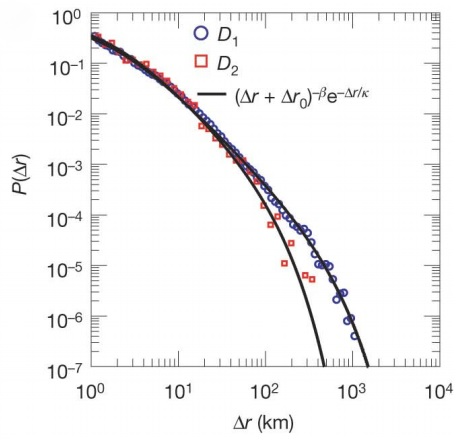
\includegraphics[scale=0.75]{truncated_power_law}
	\centering
	\caption{Truncated levy flight human motion modelling. Reproduced from \cite{Gonzalez2008}}
	\label{fig:levy_flight}
\end{figure}

This mathematical model is cited and verified in \cite{Calabrese2013}.

Methodology adopted in \cite{Hoteit2016} suggested approaches how to determine home and work locations, span of movement and complete trajectory. As already mentioned in \ref{background_mobile_location_data_sources} two datasets were compiled. The second one is a sub-sample of the first which is composed of GPS geolocation data. The sparsity of the second dataset have been mimicked by a cumulative distribution function in order to create a virtual CDR dataset. Only users with high activity were considered in order to have less irregularity. Home and work locations were determined with a mode function with catch-all time boundaries for day and night where supposedly users are either at work or home respectively. For span of movement a similar mathematical approach was adopted as the ones in \cite{Hoteit2014,Gonzalez2008} (see subsection  \ref{methodology_classification}). As for the actual movement trajectory error was calculated by calculating the euclidean distance of each CDR data-point from the actual GPS recording which is nearest in time.
Some techniques were used to lessen the margin of error. Since most of the time the typical mobile phone user is static, data completion is attained by applying a list of inference rules for which different results are achieved when estimating users location, hence the name of the paper "filling the gaps". Reader is directed to have a look at \ref{methodology_classification} for a description in detail of these refining methods. 
An issue have been raised in \cite{Calabrese2013} about detecting a lot of trips in very short distance which do not tally with statistical data given by surveys. This is explained as being cause by fluctuating random connections with towers which spatially misplace the user when in reality he is not actually physically moving. This issue was tackled by mathematically creating so called by \cite{Calabrese2013} 'virtual locations' (a mass/group of traced positions in a given radius of Airsage resolution) and actually recording a movement when user moves from a virtual location to the other. Calabrese limits static location detection to home and process how to manage to get per user is similar to that expounded in \cite{Hoteit2016}. In a novel style this work studies the relationship between total trip length calculated from mobile phone location data and vehicle kilometres travelled (VKT) and urban features such as entropic type, population density, intersection density, average distance to non-work destinations, distance to subway stations and highway exits. These urban features were derived from US Census of 2000 and activity travel surveys.


Estimation of load error is proportional to concentration if users in a given block \cite{Hoteit2014}. When error is less than 1 km a probability of 80.78\% of being within usually travelled territory contrasts with a probability of 19.22\% when user goes outside of it. When viewed from the opposite perspective the probability of being inside radius of gyration given error dimension is high is 40.25\% and that of being outside is 59.75\%.

\cite{Calabrese2013} boasts of 49.40\% of mobility variation can be explained for individual mobile users and 56.48\% for vehicle associated mobility in terms of trip length.    

In \cite{Gonzalez2008} results point to the phenomenon that the greater is the radius of gyration the less symmetric in shape is the probability density function which gives the probability of a user being in a given location (x,y). Also the margin of error increases similarly as stated in \cite{Hoteit2014}. It is also shown how individual mobility is well described by a levy-flight. Also a probability density function has been implemented to give the likelihood a user is at a certain given place in time.

The techniques used to further refine the location based on the assumed location home interval gives results in the range of 92\%-95\% of cases within 100m \cite{Hoteit2016}. Techniques will produce large errors (in the range of 50km) when user travels long distances and my not return to home location during the usual time interval.

Error distance from trajectory depends on radius of gyration \cite{Hoteit2014}. Interpolation methods are found to be most suited depending on distance from centre of mass. Nearest neighbour is most suited for $r_{g}$ less than 3 km. Between 3 km and 10 km both linear and cubic interpolations perform well. For commuting travelling patterns trajectory is best estimated with a cubic interpolation.
Interesting insights are contributed in \cite{Calabrese2013} where it is stated that job accessibility and distance to non-work destinations are inversely proportional to total trip length. Distance from subway does increase trip length for individual mobile users but it does not impact vehicle use. This means that subway commodity does not necessarily decrease vehicle use in the surrounding radius. Vehicular trip length decreases when correlated with increase in intersection density but not so for individual mobile users. Urban entropy and population does significantly impact trip length. Thus this study can help a lot in urban planning and large scale policy making.
\cite{Hoteit2016} affirms that the solution of data completion augmented by the placing of users in their home location at inferred intervals of time produces better results then what was achieved in literature.



Traffic information depends on coverage, reliability, accuracy and frequency (cite tomtom).
to compare with mobile data usage based traffic detection (accuracy 10 metres, frequency data collected every 30 sec - data sent to device every 2 minutes). 



Data privacy, Anonymization, GDPR.


Origin Destination matrices.
Clustering



Prediction methods


Evaluation methods


\begin{proof}
this is a proof
\end{proof}

\chapter{Methodology}
\section{Section Name}
insert text

\chapter{Evaluation and Results}
\section{Section Name}
insert text

\chapter{Future Work}
\section{Section Name}
insert text

\chapter{Conclusion}
insert text

\appendix

\chapter{This chapter is in the appendix}
\section{These are some details}
%%example of the code environment
\begin{code}
this is some code;
Make sure to use this template.
\end{code}


\bibliomatter
\bibliographystyle{abbrv}
 \bibliography{references}
 
\end{document}
